%%%%%%%%%%%%%%%%%%%%%%%%%%%%%%%%%%%%%%%%%
% Beamer Presentation
% LaTeX Template
% Version 1.0 (10/11/12)
%
% This template has been downloaded from:
% http://www.LaTeXTemplates.com
%
% License:
% CC BY-NC-SA 3.0 (http://creativecommons.org/licenses/by-nc-sa/3.0/)
%
%%%%%%%%%%%%%%%%%%%%%%%%%%%%%%%%%%%%%%%%%

%----------------------------------------------------------------------------------------
%	PACKAGES AND THEMES
%----------------------------------------------------------------------------------------

\documentclass{beamer}
\setbeamercovered{transparent}
\setbeamercolor{local structure}{fg=black}
\setbeamertemplate{caption}{\raggedright\insertcaption\par}
\usefonttheme[onlymath]{serif}

\mode<presentation> {
	
	% The Beamer class comes with a number of default slide themes
	% which change the colors and layouts of slides. Below this is a list
	% of all the themes, uncomment each in turn to see what they look like.
	
	%\usetheme{default}
	%\usetheme{AnnArbor}
	%\usetheme{Antibes}
	%\usetheme{Bergen}
	%\usetheme{Berkeley}
	%\usetheme{Berlin}
	%\usetheme{Boadilla}
	\usetheme{CambridgeUS}
	%\usetheme{Copenhagen}
	%\usetheme{Darmstadt}
	%\usetheme{Dresden}
	%\usetheme{Frankfurt}
	%\usetheme{Goettingen}
	%\usetheme{Hannover}
	%\usetheme{Ilmenau}
	%\usetheme{JuanLesPins}
	%\usetheme{Luebeck}
	%\usetheme{Madrid}
	%\usetheme{Malmoe}
	%\usetheme{Marburg}
	%\usetheme{Montpellier}
	%\usetheme{PaloAlto}
	%\usetheme{Pittsburgh}
	%\usetheme{Rochester}
	%\usetheme{Singapore}
	%\usetheme{Szeged}
	%\usetheme{Warsaw}
	
	% As well as themes, the Beamer class has a number of color themes
	% for any slide theme. Uncomment each of these in turn to see how it
	% changes the colors of your current slide theme.
	
	%\usecolortheme{albatross}
	%\usecolortheme{beaver}
	%\usecolortheme{beetle}
	%\usecolortheme{crane}
	%\usecolortheme{dolphin}
	%\usecolortheme{dove}
	%\usecolortheme{fly}
	%\usecolortheme{lily}
	\usecolortheme{orchid}
	%\usecolortheme{rose}
	%\usecolortheme{seagull}
	%\usecolortheme{seahorse}
	%\usecolortheme{whale}
	%\usecolortheme{wolverine}
	
	%\setbeamertemplate{footline} % To remove the footer line in all slides uncomment this line
	%\setbeamertemplate{footline}[page number] % To replace the footer line in all slides with a simple slide count uncomment this line
	
	%\setbeamertemplate{navigation symbols}{} % To remove the navigation symbols from the bottom of all slides uncomment this line
}

\usepackage{graphicx} % Allows including images
\usepackage{booktabs} % Allows the use of \toprule, \midrule and \bottomrule in tables
\usepackage{caption}
\captionsetup{font=scriptsize,labelfont=scriptsize}
\usepackage{amssymb}
\usepackage{bm}
\usepackage[colorinlistoftodos,prependcaption,textsize=small]{todonotes}                                                                                                                 

%----------------------------------------------------------------------------------------
%	TITLE PAGE
%----------------------------------------------------------------------------------------

\title[Large-Scale Data Analysis Techniques]{A Review on Multi-Label Learning Algorithms} % The short title appears at the bottom of every slide, the full title is only on the title page

\author[Sissy Themeli, Nikiforos Pittaras]{Min-Ling Zhang and Zhi-Hua Zhou} % Your name
\institute[DI-UOA] % Your institution as it will appear on the bottom of every slide, may be shorthand to save space
{
	IEEE TRANSACTIONS ON KNOWLEDGE AND DATA ENGINEERING\\ % Your institution for the title page
	\medskip
}
\date{\today} % Date, can be changed to a custom date

\begin{document}
	
	\begin{frame}
	\titlepage % Print the title page as the first slide
\end{frame}

\begin{frame}
\frametitle{Overview} % Table of contents slide, comment this block out to remove it
\tableofcontents % Throughout your presentation, if you choose to use \section{} and \subsection{} commands, these will automatically be printed on this slide as an overview of your presentation
%\setbeamercolor{section in toc}{fg=black}
%\setbeamercolor{subsection in toc}{fg=black}
\end{frame}

%----------------------------------------------------------------------------------------
%	PRESENTATION SLIDES
%----------------------------------------------------------------------------------------

%------------------------------------------------
\section{Introduction} % Sections can be created in order to organize your presentation into discrete blocks, all sections and subsections are automatically printed in the table of contents as an overview of the talk
\subsection{Problem Definition}
\begin{frame}
\frametitle{\insertsection : \insertsubsection}
Single-label supervised learning
\begin{itemize}
	\item Applied to classification
	\item Supervised: Given dataset $\{ (x_i, y_i)\}, i = 1, \dots N, x \in X, y \in Y$
	\item Goal is to learn a model $f: X \rightarrow Y$
\end{itemize}

Multi-label supervised learning
\begin{itemize}
	\item Multiple labels per instance: $\{ (x_i, \bm{y}_i)\}, i = 1, \dots N, x \in X, \bm{y} \in \mathbb{P}(Y)$
	\item Learn a model $f: X \times Y \rightarrow r$ where $r\in \mathbb{R}$ is the confidence that $y_i$ characterizes $x_i$
	\item For classification, assume that $x_i$ belongs to $y_i$ if $r$ is greater than some threshold $t(x_i)$

		\begin{itemize}
			\item $t(\cdot)$ can be a predetermined constant function or learned from $X$
		\end{itemize}

\end{itemize}
TODO: Include stuff about multi-labeled dataset characterization?
\end{frame}

%------------------------------------------------
\subsection{Algorithm Strategies}
\begin{frame}
\frametitle{\insertsection : \insertsubsection}
Label search space $\mathbb{S_Y}$ grows exponentially as a function of $|Y|$: 
\begin{itemize}
	\item e.g. for $|Y|=20, |\mathbb{S_Y}| = 2 ^ {|\mathbb{P(Y)}|} = 2^{20} \ge 10^6$
\end{itemize}
Solution: integrate in the learning process potential label correlations.
This work examines algorithms grouped in three broad categories:

\begin{enumerate}
	\item First-order strategies
		\begin{itemize}
			\item Transform multi-labeled problem to multiple, single-label problems 
			\item Ignore label correlations 
			\item Simple, scalable, suboptimal
		\end{itemize}
	\item Second-order strategies
		\begin{itemize}
			\item Consider \emph{pairwise} label relations
			\item Good trade-off between generalization performance and scalability
			\item Lacking in some real-world applications
		\end{itemize} 
	\item Higher-order strategies
		\begin{itemize}
			\item Capture more complicated label interdependencies
			\item Strong modeling capabilities
			\item Computationally demanding, less scalable
		\end{itemize}

\end{enumerate}
\end{frame}

%------------------------------------------------
\subsection{Evaluation Metrics}
\begin{frame}
\frametitle{\insertsection : \insertsubsection}
Need for more complicated evaluation than traditional supervised learning(accuracy, F-measure etc). There are 2 metrics categories 
	\begin{itemize}
		\item \emph{Example-based: }Evaluates system's performance on each example and returns the mean value. 
		\begin{itemize}
			\item \emph{From classification perspective:} $Subset Accuracy$, $Hamming Loss$, $accuracy_{exam}$, $precision_{exam}$, $recall_{exam}$, $F^\beta_{exam}$
			\item \emph{From ranking perspective:} one-error, coverage, ranking loss, average precision
		\end{itemize}
		\item \emph{Label-based: }Evaluates system's performance on each class label separately and returns macro/micro averaged value across all class labels
		\begin{itemize}
			\item From classification perspective: $B_{macro}$, $B_{micro}$
			\item From ranking perspective: $AUC_{macro}$, $AUC_{micro}$
		\end{itemize}
	\end{itemize}
TODO: theoretical results?
\end{frame}
%------------------------------------------------
\section{Multi-label Learning Algorithms}
%------------------------------------------------

\subsection{Simple Categorization}

\begin{frame}
\frametitle{\insertsection : \insertsubsection}
Algorithms in two categories:
\begin{itemize}
	\item \emph{Problem Transformation Methods: }Transform the learning problem into other well-established learning scenarios (fit data to algorithm philosophy)
	\item \emph{Algorithm Adaptation Methods: }Adapt popular learning techniques to deal with multi-label data directly (fit algorithm to data philosophy)
\end{itemize}
\begin{figure}
	\begin{center}
		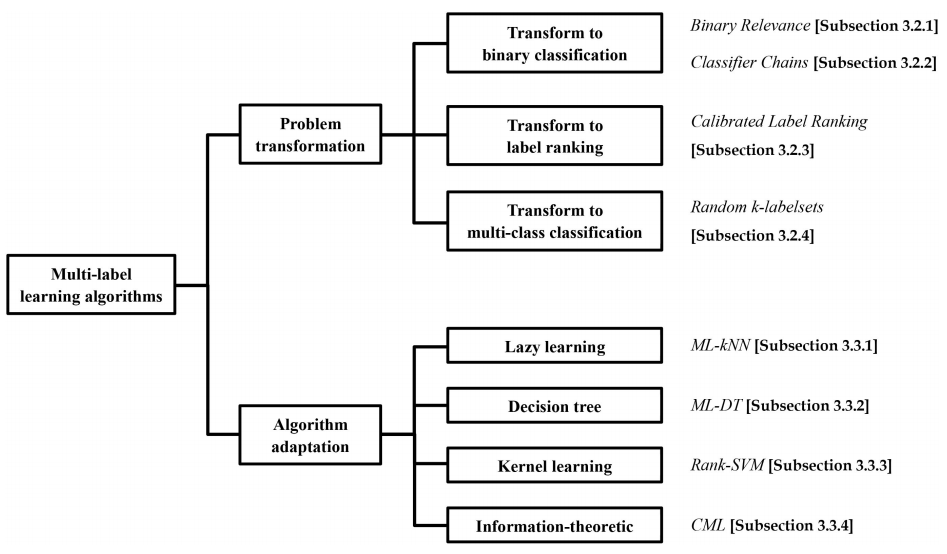
\includegraphics[scale = 0.25]{images/algorithmsclass.png}
		\caption{8 representative algorithms}
	\end{center}
\end{figure}
\end{frame}

%------------------------------------------------
\subsection{Problem Transformation Methods}

\begin{frame}
\frametitle{\insertsection : \insertsubsection}
\emph{Binary Relevance}
\begin{itemize}
	\item Decompose problem into q independent binary classification problems per possible label in the label space
\end{itemize}

\end{frame}
%------------------------------------------------

\begin{frame}
\frametitle{Classifier chains}
\begin{itemize}
\item <2-> 
\begin{itemize}
\item 
\item <4-> 
\end{itemize}
\end{itemize}
\begin{itemize}
\item<5-> 
\end{itemize}

\begin{itemize}
\item <7-> 
\begin{itemize}
\item <8-> 
\end{itemize}
\end{itemize}
\end{frame}
%------------------------------------------------

\begin{frame}
\frametitle{Calibrated Label Ranking}
\begin{itemize}
\item <2-> 
\begin{itemize}
\item 
\item <4-> 
\end{itemize}
\end{itemize}
\begin{itemize}
\item<5-> 
\end{itemize}

\begin{itemize}
\item <7-> 
\begin{itemize}
\item <8-> 
\end{itemize}
\end{itemize}
\end{frame}
%------------------------------------------------
\begin{frame}
\frametitle{Random k-Labelsets}
\begin{itemize}
\item <2-> 
\begin{itemize}
\item 
\item <4-> 
\end{itemize}
\end{itemize}
\begin{itemize}
\item<5-> 
\end{itemize}

\begin{itemize}
\item <7-> 
\begin{itemize}
\item <8-> 
\end{itemize}
\end{itemize}
\end{frame}
%------------------------------------------------

\subsection{Alogrithm Adaptation Methods}

\begin{frame}
\frametitle{Multi-Label k-Nearest Neighbor}
\begin{itemize}
\item <2-> 
\item <3-> 
\item <4-> 
\item<5-> 
\item <6-> 
% \item<7->
\end{itemize}
\end{frame}

%------------------------------------------------
\begin{frame}
\frametitle{Multi-label Decision Tree}

%\begin{figure}
%	\includegraphics[width = \textwidth, height = \textheight, keepaspectratio]{modelcharacters.png}
%	\caption{Character enhanced word representations}
%	\end{figure}
\end{frame}
%------------------------------------------------
\begin{frame}
\frametitle{Ranking Support Vector Machine}

%\begin{figure}
%	\includegraphics[width = \textwidth, height = \textheight, keepaspectratio]{modelcharacters.png}
%	\caption{Character enhanced word representations}
%	\end{figure}
\end{frame}
%------------------------------------------------
\begin{frame}
\frametitle{Collective Multi-Label Classifier}

%\begin{figure}
%	\includegraphics[width = \textwidth, height = \textheight, keepaspectratio]{modelcharacters.png}
%	\caption{Character enhanced word representations}
%	\end{figure}
\end{frame}
%------------------------------------------------
\section{Related Learning Settings}
%------------------------------------------------

\begin{frame}
\frametitle{Related Learning Settings}
\begin{itemize}
\item 
\item 
\item 
\item 
\end{itemize}
\end{frame}

%------------------------------------------------
\section{Conclusion}
%------------------------------------------------
\begin{frame}
\frametitle{Conclusion}
\begin{itemize}
\item 
\item 
\end{itemize}
\onslide<4->{}
\begin{itemize}
\item <5-> 
\item <6->
\item <7-> 
\end{itemize}
\end{frame}

%------------------------------------------------
\section{The end}
\begin{frame}
\Huge{\centerline{Thank you}}
\end{frame}

%------------------------------------------------

\end{document} 
